To convey the commands from the transmitter to the receiver, a wireless connection is needed, in this case
implemented through two HC-05 modules. These boards are, in technical terms, Bluetooth SPP (Serial Port Protocol) modules, used to abstract the wireless connection implementation.\\

\begin{figure}[H]
	\hspace*{0.3 \textwidth}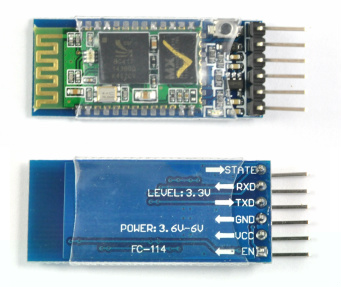
\includegraphics[width= 0.4\textwidth]
	{files/images/hc05_view}
	\caption{View of the HC-05 surfaces.}
\end{figure}

\subsection{Command and Data Transfer modes}
This module has two modes of operation:
\begin{itemize}
	\item \textit{Command Mode} (or \textit{AT Mode}): used for configuring the module (through AT commands);
	\item \textit{Data Mode}: used for transmitting and receiving data to/from another Bluetooth module.
\end{itemize}

\subsection{Default settings}
The default settings for new modules are:
\begin{itemize}
	\item Device name: HC-05;
	\item Password: 1234;
	\item Baud rate in communication mode: 9600 characters per second (but sometimes 38400 characters per second);
	\item Baud rate in \textit{AT Mode}: 38400 characters per second;
	\item State: there are two possible states for this module, master and slave, the second is the default behaviour.
\end{itemize}
The default device mode is the \textit{Data Mode} and it is used to broadcast data through Bluetooth.\\

\subsection{\textit{AT Mode}}
AT command mode allows to interrogate and to modify the previous settings described. Changing the module state, it is possible to configure it to automatically connect to another Bluetooth device, as it will be made in this project.\\
To use the Command mode, an USB to TTL adapter or an opportunely configured Arduino board is needed. The HC05 should be connected to one of these devices according to the following scheme:\\

\begin{tabular}{|c|c|c|}
	\hline 
	\textbf{HC-05 pin} & \textbf{For \textit{USB to TTL}} & \textbf{For \textit{Arduino}} \\ 
	\hline 
	(1) +5V & Vcc & Vcc \\ 
	\hline 
	(2) GND & GND & GND \\ 
	\hline 
	(3) Tx & Rx & Rx \\ 
	\hline 
	(4) Rx & Tx & Tx \\ 
	\hline 
\end{tabular}

\subsubsection{Enter in \textit{AT Mode} through EN pin}
\begin{figure}[H]
	\hspace*{0.3 \textwidth}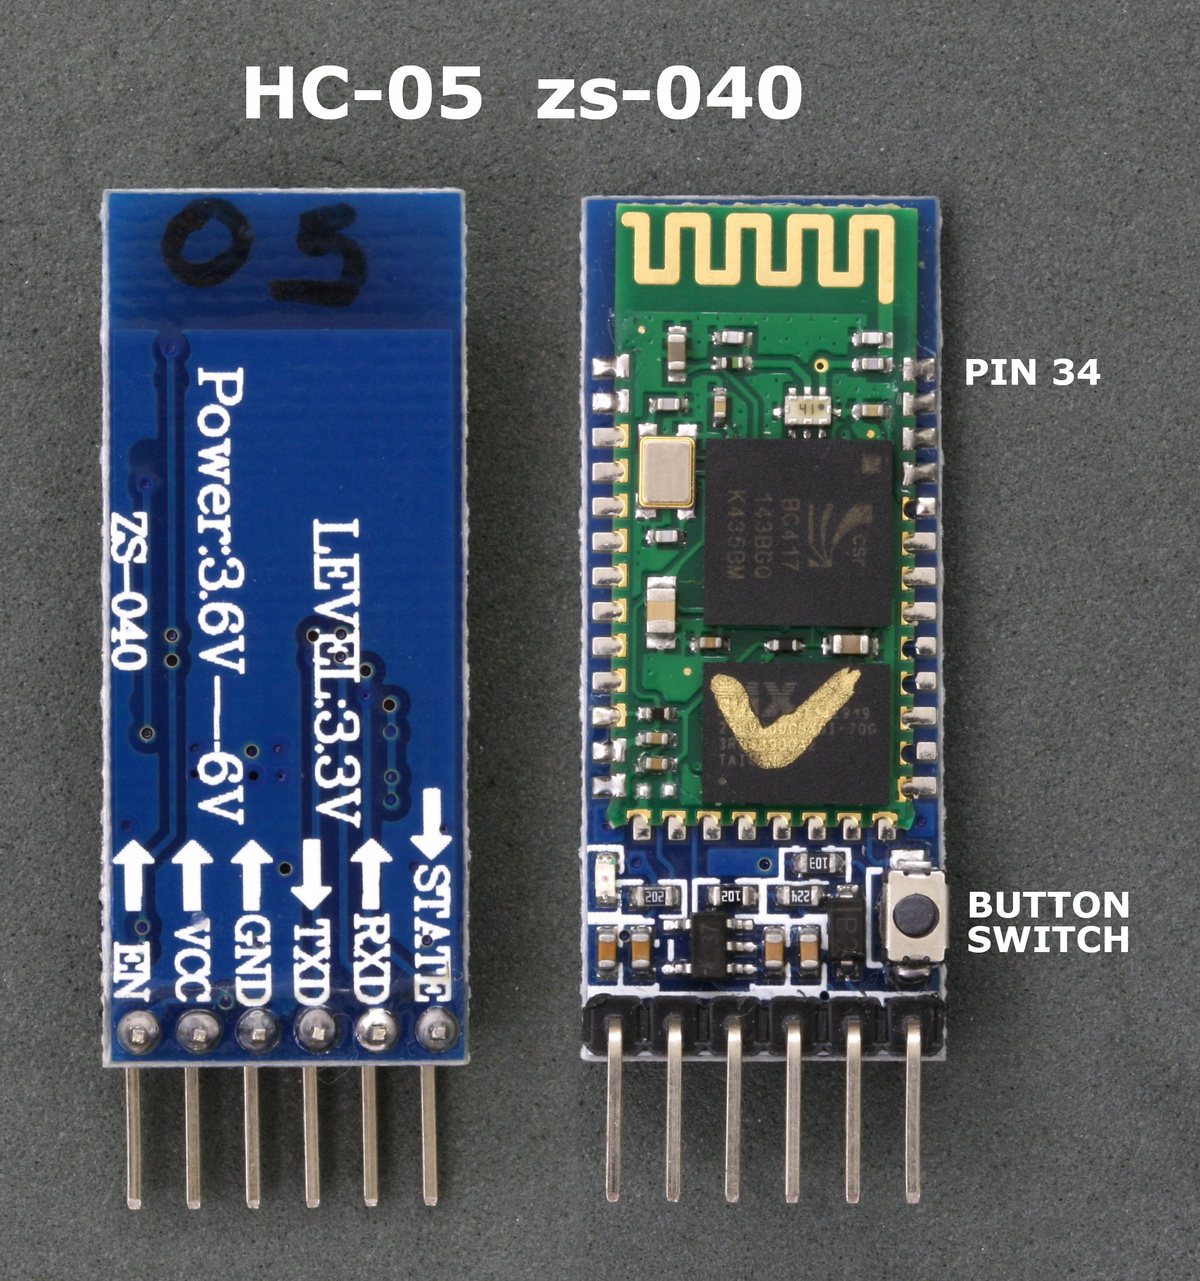
\includegraphics[width= 0.4\textwidth]
	{files/images/hc05_en_pin}
	\caption{HC-05 module with EN pin and button switch.}
\end{figure}
To activate \textit{AT Mode} on these HC-05 modules, the pin 34 has to be high on power up. For this purpose there are two different approaches: \begin{itemize}
\item if there is a button on the module, press it: this will automatically connect the pin 34 to the high power source
\item if not, manually connect pin 34 to a 5V voltage source through a jumper wire.
\end{itemize}
To enter this mode, the pin 34 must be connected to at least 4V when powering on the module. Once the module has booted, the voltage on pin 34 can become high impedance.\\
To verify if the module is in \textit{AT Mode}, the LED on the HC05 should blink with halved frequency.

\subsection{Setup the communication}
Once the HC-05 is in \textit{AT Mode}, the module can be configured through the \textit{Arduino Serial Module}. The configuration will require that both \textit{NL} and \textit{CR} as end line are enabled and the communication will be kept at 38400 characters per second.\\
It is necessary to set the two modules, one for the master role and one for the slave one, since the two modules should connect to each other automatically, without the support of the boards. The master will seek a Bluetooth module (the slave) whose address is the given one, and will establish the connection.

\subsubsection{Slave configuration}
The slave mode will be used on the Arduino:
\begin{enumerate}
	\item Boot the HC05 in \textit{AT Mode} and connect it to the Arduino;
	\item To verify if the connection is right, it is possible to type \textit{AT}, which should return \textit{OK};
	\item Typing \textit{AT+UART?}, the module will answer with the actual baud rate, which should be 9600 characters per second, compatible with the Arduino serial port;
	\item Typing \textit{AT+ROLE?}, the module should answer a message like \textit{+ROLE=0}, which means that the Bluetooth device is in slave mode;
	\item Typing \textit{AT+ADDR?}, the module should answer with its address, like 18:e4:34cldd, and it is necessary to use this to configure the master module.
\end{enumerate}

\begin{figure}[H]
	\hspace*{0.1 \textwidth}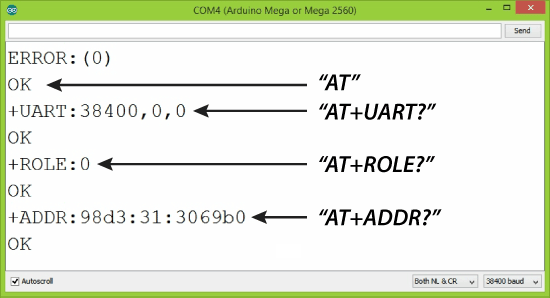
\includegraphics[width= 0.8\textwidth]
	{files/images/hc05_slave2}
	\caption{Slave configuration of the HC-05 module trough serial monitor.}
\end{figure}

\subsubsection{Master configuration}
The master module will be used on the Discovery board. The configuration process is similar to the previous module so here only the relevant commands will be explained.\\
\begin{enumerate}
	\item Boot the HC05 in \textit{AT Mode} and connect it to the Arduino;
	\item The STM32F407 uses \textit{9600} baud rate to communicate on USART2, so it is necessary to change the hc-05 baud rate, through the command \textit{AT+UART=9600,0,0};
	\item Typing \textit{“AT+ROLE=1”}, the serial device will set the Bluetooth module as a master device;
	\item Typing \textit{AT+CMODE=0} the serial device will set the connection mode as \textit{fixed address} and, using the \textit{AT+BIND=XX,XXXX,XX} command, putting there the slave address, the master will be set to search this module and connect there (in the address specification it is required using commas, instead of colons).
\end{enumerate}

\begin{figure}[H]
	\hspace*{0.1 \textwidth}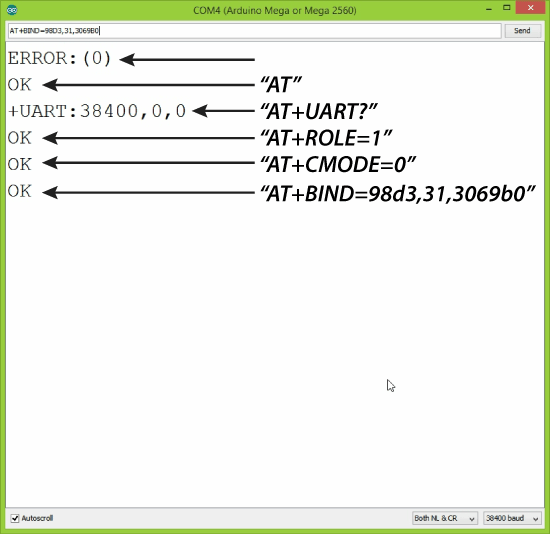
\includegraphics[width= 0.8\textwidth]
	{files/images/hc05_master}
	\caption{Master configuration of the HC-05 module trough serial monitor.}
\end{figure}
 \newpage
 
 \subsection{The communication to the HC05 modules}
 
\subsubsection{The transmitter}
The code on the Discovery uses the USART2 channel to communicate with the connected HC-05 module.\\
So, it is necessary to link the HC-05 \textit{Rx} pin to Discovery PA2 pin (USART2 \textit{TX}) and HC-05 \textit{Tx} pin to PA3 (USART2 \textit{RX})\\
In this project, the Discovery only send strings to Arduino, so the code will only write on the PA2 pin but the implementation regards also the contrary stream for future expansions. To send a string, it is just require to use the \textit{printf} function implemented in the Miosix kernel.\\

\subsubsection{The receiver}
The project uses the pin 12 (\textit{TX}) and the pin 11 (\textit{RX}) to communicate with the HC-05 module. To read a string from the HC-05 on Arduino is enough to use the \textit{read()} function of the SoftwareSerial class.\\